\documentclass[10pt]{article}
\usepackage[a4paper,margin=2.0cm]{geometry}
\usepackage[T1]{fontenc}
\usepackage{lmodern}
\usepackage{microtype}
\usepackage{amsmath}
\usepackage{booktabs}
\usepackage{graphicx}
\usepackage{caption}
\usepackage{float}
\usepackage[hidelinks]{hyperref}
\graphicspath{{figures/}}
\setlength{\parskip}{0.45em}
\setlength{\parindent}{0pt}
\captionsetup{font=small,labelfont=bf}

\title{\vspace{-1.6em}Effect of video compression on the leaf weights:\\ sensitivity of the rendered error to codec, bitrate and quantization}
\author{}
\date{\vspace{-2.4em}}

\begin{document}
\maketitle
\vspace{-1.0em}

\textbf{Summary.} Leaf weights taken from lossy encodes change the rendered error by at most 3\% (0.23\,dB of PSNR) with respect to exact leaf weights, across VP9, HEVC and AV1 and across bitrates from 74 down to 0.6\,Mb/s (decoded PSNR from 51 down to 32\,dB). There is no trend with bitrate. Quantizing the block mean directly changes the error by about 3\% at most, up to a step of 64 of 1023 code values. The estimator stays unbiased throughout; compression only changes its variance.

\section*{1\quad Why compression changes variance, not the expected value}

The leaf weights define the sampling pdf (Eq.~2 of the paper), so an error in a weight changes the pdf, as the reviewer points out. The light estimator divides each sample by the pdf actually used, so it is unbiased for any pdf that is positive wherever the emitter radiance is positive. A misestimated weight therefore cannot bias the image; it can only increase variance, by making the pdf a worse match for the radiance. The one way to introduce bias would be a weight quantized to zero over a leaf whose radiance is not zero. The weights used here keep a small density floor ($10^{-4}$ of the mean weight) to prevent it. So the question is quantitative: how much variance does compression add? The experiment below measures it.

\section*{2\quad From the coded stream to leaf radiance}

In a block transform codec, the DC coefficient of a block, divided by the transform gain, is the mean of that block of the coded plane. For a block coded with prediction, the reconstructed block mean is the mean of the prediction plus the dequantized DC of the residual; the residual's DC alone is not the block mean. We obtain the mean of each leaf in the reconstructed 10-bit PQ Y$'$, Cb and Cr planes, which is the value this DC computation gives after quantization, and turn it into a weight in three steps: (1) convert the means to $R'G'B'$ with the BT.2020 matrix; (2) apply the PQ EOTF (BT.2100) and take luminance with BT.2020 weights; (3) multiply by the leaf area. The EOTF of a mean slightly underestimates the mean of the EOTF; Table~\ref{tab:emul} shows that this, and using Y$'$ alone, cost at most about 2\%.

\section*{3\quad Setup}

Five scenes of the paper (Rover, Cinema, Fireplace, Phone, Convergence), one frame each. Each frame is coded as an inter frame in the middle of a 9-frame window of its video, in 10-bit PQ at its native resolution. Encoders (ffmpeg): libvpx-vp9 (profile 2) at CRF 12, 32, 48 and 63; x265 at CRF 18, 28 and 40; SVT-AV1 at CRF 25, 40 and 55. The partition is the CodecLeafAlias partition of the paper. Every configuration is rendered in our GPU path tracer at equal samples (4 spp; 16 in Phone), 32 independent captures, and compared with a converged reference. We report the RMSE relative to the RMSE obtained with exact leaf weights (the linear mean of the source frame over each leaf) on the same partition. The 95\% confidence half-width of that baseline is 2.4, 0.8, 0.3, 2.1 and 0.1\% in Rover, Cinema, Fireplace, Phone and Convergence.

\section*{4\quad Results}

\begin{table}[H]
\centering\small
\begin{tabular}{lcccccccc}
\toprule
& Bitrate (Mb/s) & PSNR Y$'$ (dB) & \multicolumn{5}{c}{RMSE / RMSE with exact weights} & Max PSNR \\
\cmidrule(lr){4-8}
Encode & mean [range] & mean & Rover & Cinema & Fire. & Phone & Conv. & loss (dB) \\
\midrule
VP9, CRF 12 & 35.3 [17.7--74.4] & 50.4 & 1.003 & 1.002 & 1.001 & 1.004 & 0.996 & 0.03 \\
VP9, CRF 32 & 10.5 [6.0--23.7] & 44.3 & 1.005 & 1.002 & 1.003 & 1.004 & 0.996 & 0.04 \\
VP9, CRF 48 & 3.3 [2.1--6.8] & 39.3 & 1.020 & 1.007 & 1.002 & 1.015 & 0.996 & 0.17 \\
VP9, CRF 63 & 0.9 [0.6--1.6] & 34.8 & 1.015 & 1.005 & 1.005 & 1.014 & 0.999 & 0.12 \\
\midrule
HEVC, CRF 18 & 16.8 [8.5--39.7] & 46.9 & 1.009 & 1.003 & 1.003 & 1.010 & 0.995 & 0.08 \\
HEVC, CRF 28 & 4.9 [2.4--12.1] & 41.6 & 1.015 & 1.005 & 1.003 & 1.014 & 0.996 & 0.12 \\
HEVC, CRF 40 & 1.0 [0.6--2.2] & 35.6 & 1.003 & 1.001 & 1.004 & 1.007 & 0.997 & 0.06 \\
\midrule
AV1, CRF 25 & 11.4 [5.9--27.9] & 45.6 & 1.003 & 1.000 & 1.002 & 1.006 & 0.997 & 0.06 \\
AV1, CRF 40 & 4.1 [2.1--9.0] & 41.5 & 1.018 & 1.007 & 1.003 & 1.016 & 0.996 & 0.15 \\
AV1, CRF 55 & 1.5 [0.7--3.0] & 37.7 & 1.029 & 1.011 & 1.006 & 1.028 & 0.997 & 0.23 \\
\bottomrule
\end{tabular}
\caption{Real encodes. Bitrate at 24\,fps and decoded PSNR of Y$'$ across the five scenes; RMSE of the rendered frame with weights from the decoded stream, relative to exact weights; largest PSNR loss over the five scenes.}
\label{tab:real}
\end{table}

\begin{figure}[H]
\centering
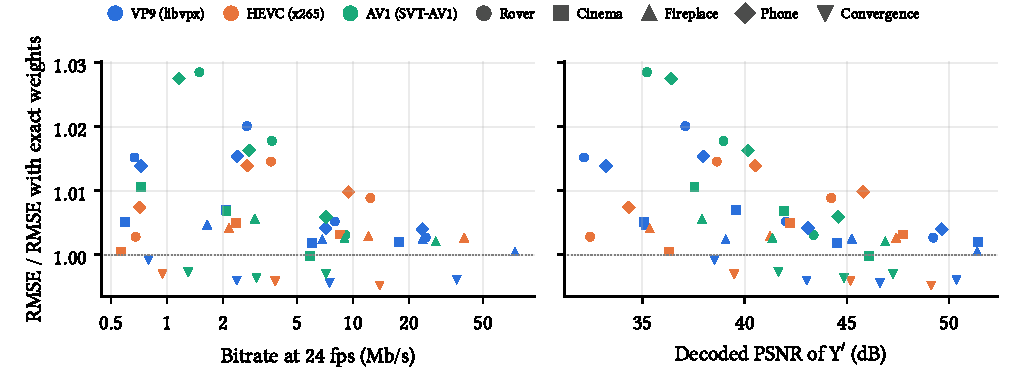
\includegraphics[width=\linewidth]{rate_sensitivity.pdf}
\caption{The data of Table~\ref{tab:real} against bitrate (left) and decoded PSNR (right). All 50 points lie between 0.995 and 1.029, with no trend toward low bitrates.}
\label{fig:rate}
\end{figure}

\textbf{Bitrate and QP.} Every ratio lies between 0.995 and 1.029, and the largest PSNR loss is 0.23\,dB, at the lowest AV1 rate. The ratios do not grow as the bitrate falls: the lowest VP9 and HEVC rates (0.6--2.2\,Mb/s, about 35\,dB) are as good as the highest. Deviations are largest in Rover and Phone, which also have the widest confidence intervals ($\pm$2.4\% and $\pm$2.1\%). Compression error is spread over each block, while a leaf weight is the mean over the whole leaf, so most of it averages out.

\textbf{Codec.} VP9, HEVC and AV1 behave alike: their worst ratios are 1.020, 1.015 and 1.029. Nothing in the method depends on VP9.

\textbf{Partition from the decoded frame.} A decoder only sees the decoded frame. Taking the partition from it instead of from the source changes the ratios to 0.996--1.019, also with no trend in bitrate.

\begin{table}[H]
\centering\small
\begin{tabular}{llccccc}
\toprule
Partition & Leaf weight & Rover & Cinema & Fireplace & Phone & Convergence \\
\midrule
Codec & PQ Y$'$ mean only & 1.008 & 1.004 & 1.004 & 0.999 & 0.985 \\
& PQ Y$'$CbCr means & 1.004 & 1.001 & 1.001 & 0.998 & 0.996 \\
& mean quantized, step 4 & 0.994 & 0.998 & 1.001 & 0.991 & 0.996 \\
& mean quantized, step 16 & 1.017 & 1.006 & 1.002 & 1.012 & 0.997 \\
& mean quantized, step 64 & 1.011 & 1.006 & 1.011 & 1.014 & 1.000 \\
& mean quantized, step 256 & 1.050 & 1.041 & 1.080 & 1.070 & 1.132 \\
\midrule
Budget, 4000 leaves & PQ Y$'$CbCr means & 0.993 & 0.996 & 1.022 & 1.007 & 0.989 \\
& mean quantized, step 16 & 1.007 & 1.003 & 1.022 & 1.016 & 0.989 \\
& mean quantized, step 64 & 1.016 & 1.007 & 1.031 & 1.024 & 0.995 \\
& mean quantized, step 256 & 1.051 & 1.037 & 1.106 & 1.076 & 1.099 \\
\bottomrule
\end{tabular}
\caption{Nonlinearity and direct quantization of the block mean, in 10-bit PQ code values (step $s$ of 1023, applied to each of Y$'$, Cb and Cr), on the same frames. RMSE relative to exact linear weights on the same partition.}
\label{tab:emul}
\end{table}

\textbf{Quantization step.} Quantizing the block means directly (Table~\ref{tab:emul}) isolates the reviewer's mechanism from everything else a codec does. Up to a step of 64 code values, a sixteenth of the range, the error grows by about 3\% at most, for both partitions. Only a step of 256, a quarter of the range, reaches 4--13\%.

\textbf{Reading the residual alone does not work.} If the DC of a predicted block's residual is taken as the block mean, without adding the prediction's mean, the weights are wrong and the RMSE grows 1.1--3.5$\times$. The prediction must be included, as described in Section~2.

\begin{figure}[H]
\centering
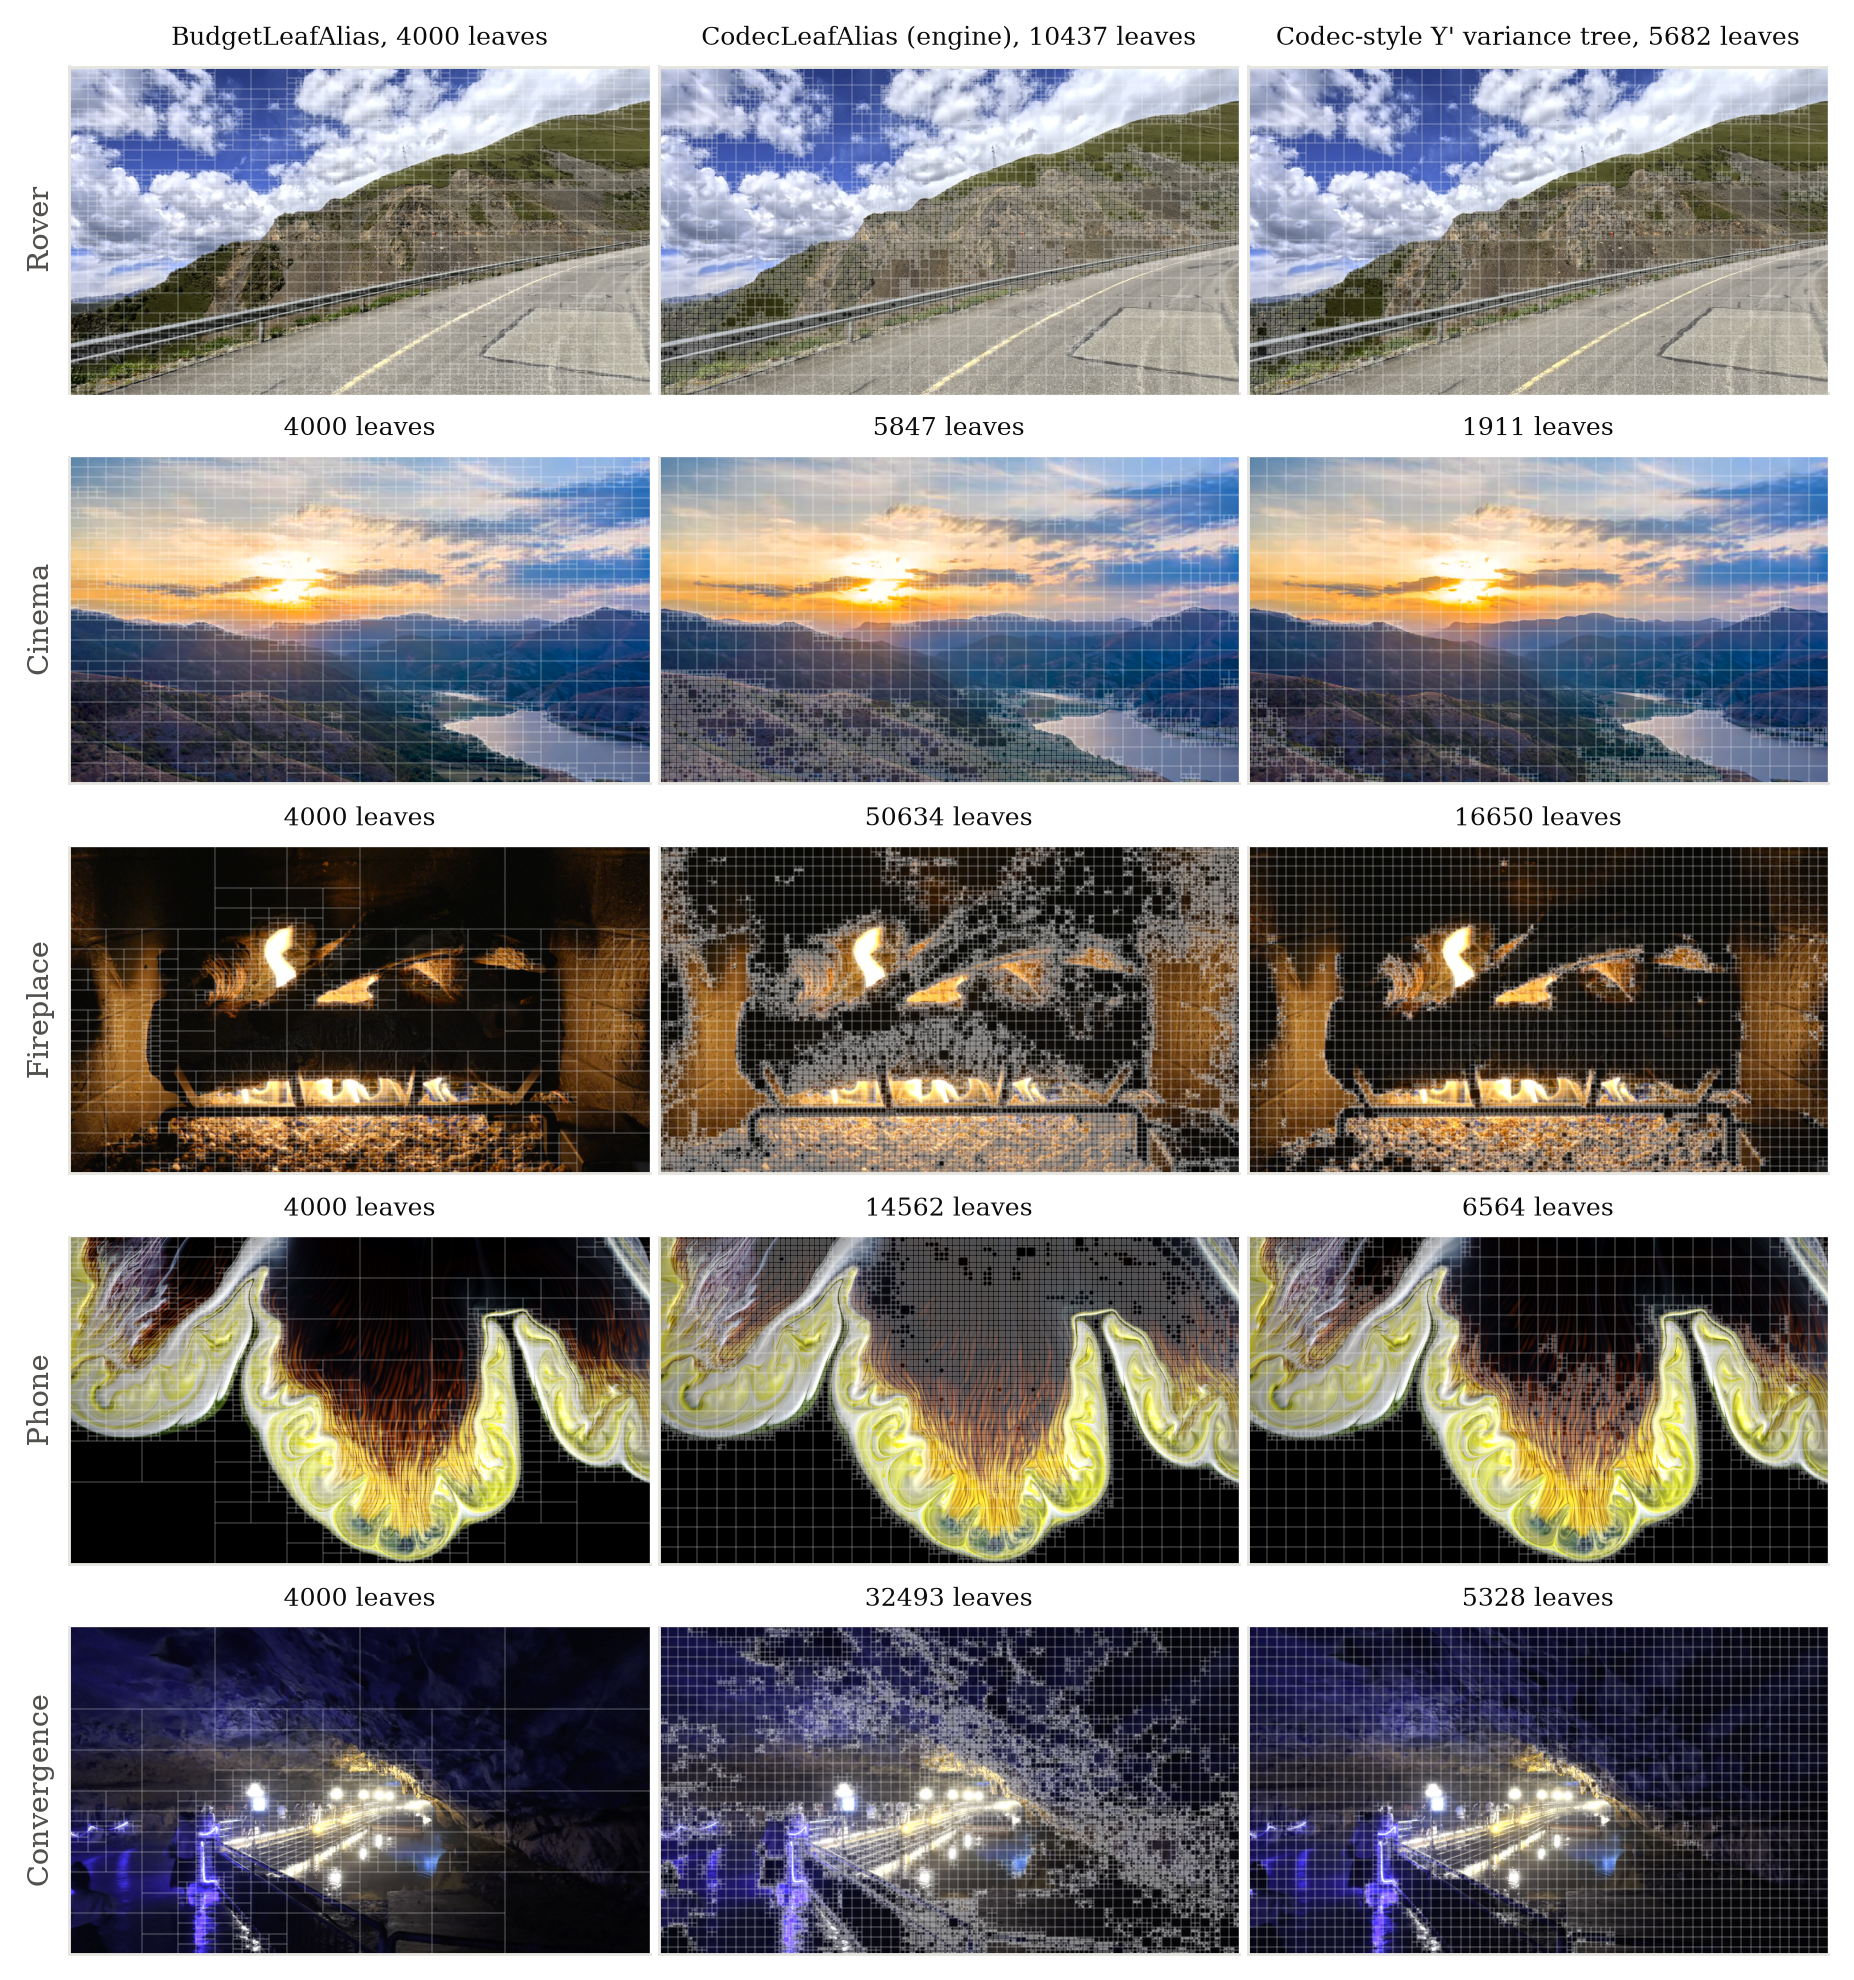
\includegraphics[width=0.6\linewidth]{partitions_side_by_side.png}
\caption{Leaf partitions of the five scenes: BudgetLeafAlias with 4000 leaves, the CodecLeafAlias partition used in this experiment, and a codec-style variance tree on Y$'$.}
\label{fig:parts}
\end{figure}

\section*{5\quad Conclusion}

Compression changes the pdf but cannot bias the estimate, and the variance it adds is small: at most 3\% RMSE, or 0.23\,dB of PSNR, over three codecs and ten rate points from 74 to 0.6\,Mb/s, with no dependence on bitrate. The same holds when the block mean is quantized directly, up to a step of 64 of 1023. The method is not tied to VP9: HEVC and AV1 give the same result.

\end{document}
